\documentclass[onecolumn]{aastex62}


\newcommand{\vdag}{(v)^\dagger}
\newcommand\aastex{AAS\TeX}
\newcommand\latex{La\TeX}
\usepackage{listings}
\usepackage{amsmath}
\usepackage{physics}
\usepackage{hyperref}
\usepackage{natbib}
\usepackage[T1]{fontenc}
\usepackage[english]{babel}
\usepackage[utf8]{inputenc}

\begin{document}

\title{\Large Milestone II:\\Studying the recombination history of the universe.}


\author{Håkon Tansem}

\section{Introduction} \label{sec:intro}
This is the second out of four milestones in a project where the final goal is to compute the CMB power spectrum. Previously we calculated the background evolution of the universe studying how the energy content and the particle horizon has evolved throughout cosmic history. Another important consideration to take into account when observing the CMB is to study the medium the photons have travelled from their release at the last scattering surface untill they reach us at present time. In this second milestone we will study how the optical depth of the universe changes as we look further back in time. To do this we will have to study the recombination history of the universe; i.e how the fraction of ionized matter versus neutral matter has changed during the history of the universe. 
\section{Method} \label{sec:method}
The general expression for optical depth $\tau$ is given by
\begin{equation}
    d\tau\equiv\alpha(s)ds,
\end{equation}
where $\alpha(s)$ is the attenuation coefficient and $s$ is the thickness of the medium. When considering the intergalactic medium the CMB photons have traversed untill we observe them, the main contributor to the attenuation coefficient is thomson scattering off free electrons. The expression for optical depth $\tau$ can be written as
\begin{equation}
    d\tau=n_e\sigma_T ad\eta,
\end{equation}
where $n_e$ is the free electron density, $\sigma_T = \frac{8\pi}{3}\frac{\alpha^2\hbar^2}{m_e^2c^2}$ is the Thomson scattering cross-section,$\alpha$ is the fine structure constant and $a$ is the scale factor. We have now also changed coordinates to the conformal time $\eta$ representing the thickness of the medium. By performing a change of coordinates to $x=log(a)$ we can get a differential equation for $\tau$ given By
\begin{equation}\label{eq:optical_depth_of_x}
    \frac{d\tau}{dx} = -\frac{n_e \sigma_T }{H(x)},
\end{equation}
where $H(x)$ is the Hubble parameter in our new coordinate system. The evolution of the Hubble parameter used in the calculation is described in milestoneI. To solve the ODE for $\tau$ we need to evaluate the electron density $n_e$ as a function of $x=log(a)$. When studying the recombination history of the universe, our model will include some simplifications. In this project we will mostly study the phenomenon of recombination and ignore the recombionization the universe went through later. We assume the universe mostly consists of hydrogen by setting the helium fraction $Y_p=0$. We also assume that all baryonic matter is represented by the hydrogen nucleus. This makes us able to approximate the proton density $n_H$ as
\begin{equation}\label{eq:baryondensity}
    n_H = n_b \approx \frac{\rho_b}{m_H} = \frac{\Omega_{b,0} \rho_{c,0}}{m_H a^3},
\end{equation}
where $n_b$ is the baryon density, $\rho_{c,0}$ is the critical density of the universe today, $\Omega_{b,0}$ is the density parameter for baryons today and $m_H$ is the hyodrogen mass. A relationship between the quantities $n_e$ and $n_H$ can be expressed through the free electron fraction given by

\begin{equation}\label{eq:Xe}
    X_e\equiv\frac{n_e}{n_H}.
\end{equation}
 
This allows us to solve for $n_e$ to compute the optical depth given in equation \ref{eq:optical_depth_of_x}. The free electron fraction can be solved using two equations dependent on quantities that evolve with $x=log(a)$. The first one is the Saha equation given by
\begin{equation}\label{eq:saha_eq}
    \frac{X_e^2}{1-X_e} = \frac{1}{n_b} \left(\frac{m_eT_b}{2\pi}\right)^{3/2} e^{-\epsilon_0/T_b},
\end{equation}
where $\epsilon_0=13.6$eV is the ionization energy of the hydrogen atom, $m_e$ is the electron mass and $T_b$ is the baryon temperature. The baryon temperature can be approximated by the photon temperature giving $T_b =
T_r = T_{\rm CMB} / a = 2.725 \textrm{K} / a$ \cite{WintherII:2020}. The second equation one can use to solve for the free electron fraction is the Peebles' equation given by
\begin{equation}\label{eq:peeble_eq}
    \frac{dX_e}{dx} = \frac{C_r(T_b)}{H(x)} \left[\beta(T_b)(1-X_e) - n_H\alpha^{(2)}(T_b)X_e^2\right],
\end{equation}
where the reaction rates are given by
\begin{align}
    C_r(T_b) &= \frac{\Lambda_{2s\rightarrow1s} +
    \Lambda_{\alpha}}{\Lambda_{2s\rightarrow1s} + \Lambda_{\alpha} +
    \beta^{(2)}(T_b)}, \\
    \Lambda_{2s\rightarrow1s} &= 8.227 \textrm{s}^{-1}\\
    \Lambda_{\alpha} &= H\frac{(3\epsilon_0)^3}{(8\pi)^2 n_{1s}}\\
    n_{1s} &= (1-X_e)n_H \\
    \beta^{(2)}(T_b) &= \beta(T_b) e^{3\epsilon_0/4T_b} \\
    \beta(T_b) &= \alpha^{(2)}(T_b) \left(\frac{m_e
    T_b}{2\pi}\right)^{3/2} e^{-\epsilon_0/T_b} \\
    \alpha^{(2)}(T_b) &= \frac{64\pi}{\sqrt{27\pi}}
    \frac{\alpha^2}{m_e^2}\sqrt{\frac{\epsilon_0}{T_b}}\phi_2(T_b) \\
    \phi_2(T_b) &= 0.448\ln(\epsilon_0/T_b)
\end{align}
\cite{WintherII:2020}. The Saha equation given by equation \ref{eq:saha_eq} is derived with the assumption that we have the equilibrium reaction $e^- +p\rightleftharpoons H+\gamma$ \cite[p.70]{Dodelson:1282338}. That is the relation between free electrons and protons and neutral hydrogen remains relatively constant. In this case of the early universe all matter is ionized making this a reasonable condition. Thus this equation is only valid as long as the free electron fraction $X_e$ is close to one. Therefore we solve we solve the Saha equation when $1\leq X_e<0.99$. This equation can be solved as a regular second order equation where the solution is given by
\begin{equation}
    X_e = \frac{F(x)}{2}\left[-1\pm\sqrt{1+4/F(x)}\right],
\end{equation}
where $F=\frac{1}{n_b} \left(\frac{m_eT_b}{2\pi}\right)^{3/2} e^{-\epsilon_0/T_b}$. Here we only take into account the positive solution as the negative solution has no physical importance. we have to resort to the Peebles' equation given by equation \ref{eq:peeble_eq}. Using a numerical ODE solver one can solve the peebles equation from $x_{transition}$ untill today where $x_{transition}$ is first $x$ value where $X_e$ is less than $0.99$. Since the solutions for $X_e$ and $n_e$ varies several orders of magnitude over a relatively short time period, we spline the logarithm of the solution to reduce numerical errors.
\\\\\indent
Now that we can evaluate $n_e$ for an arbitrary $x$ we can solve the ODE for tau given by equation \ref{eq:optical_depth_of_x} numerically. From the definition of the optical depth, we know that the boundary condition implies that at current time $\tau=0$. When looking at $x=0$ we haven't looked back in time through any of the intergalactic so there is so significant attenuation. Since we do not know the boundary condition as $x$ approaches infinity we set an arbitrarily large initial value for $\tau$. In this case $\tau_0=10^5$ was chosen. We can then subtract the solution at $x=0$ from the whole solution scaling it properly so that it reaches zero today. The final quantity we will compute is the visibility function given by
\begin{equation}\label{eq:visibility}
    \widetilde{g}(x)=-\frac{d\tau}{dx}e^{-\tau}.
\end{equation}
This quantity is normalized as
\begin{equation}
    \int_{-\infty}^{0} \tilde{g}(x)dx = 1,
\end{equation}
making it a probability distribution. It describes the probability at which $x$ an observed CMB photon observed today was last scattered (\cite{callin2006calculate}).
\section{Results}
\label{sec:results}
By combining the Saha equation and Peebles' equation given by equations \ref{eq:saha_eq} and \ref{eq:peeble_eq} respectively, as described in section \ref{sec:method} the free electron fraction $X_e$ was calculated. This is shown in figure \ref{fig:xe}. The resulting electron density calculated by equations \ref{eq:baryondensity} and \ref{eq:Xe} is shown in figure \ref{fig:ne}. By defining the time of recombination to be the point at which $X_e=0.5$, we find the closest point in our simulation to be $x=-7.16$, which corresponds to a redshift of approximately $z=1293$.
\begin{figure}
    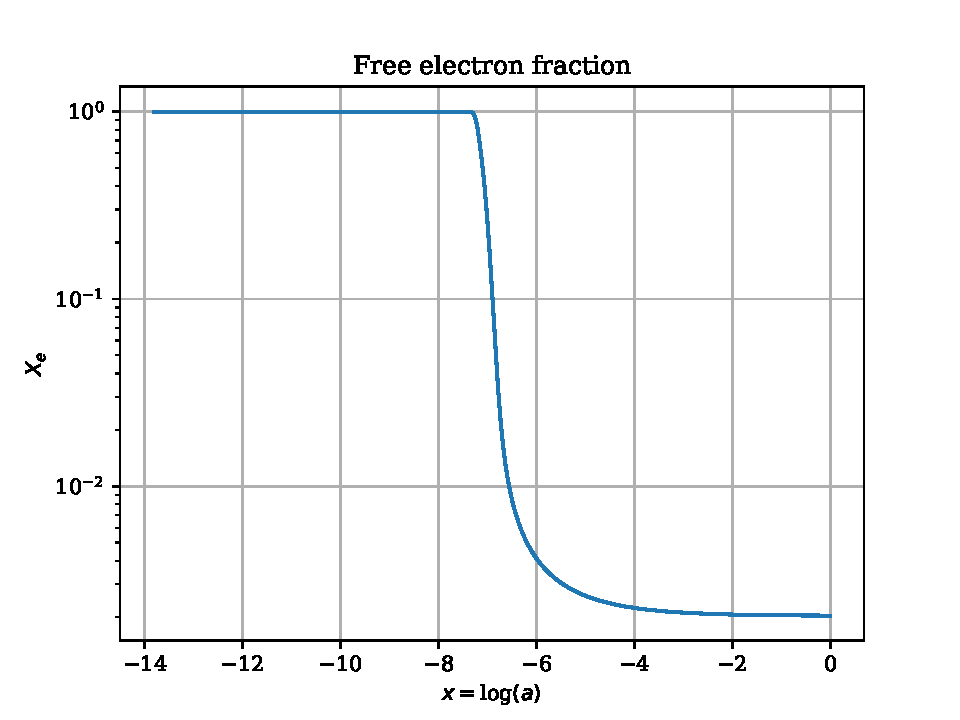
\includegraphics[scale=0.8]{figures/xe.pdf}
    \caption{Figure showing the free electron fraction $X_e$ as a function of $x=log(a)$.}
    \label{fig:xe}
\end{figure}

\begin{figure}
    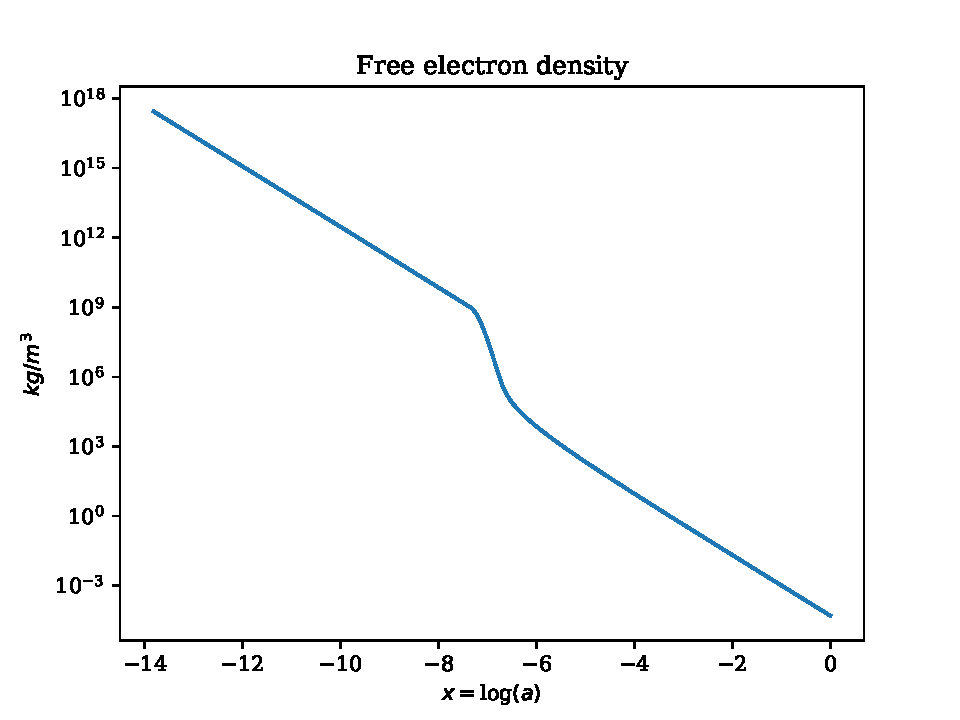
\includegraphics[scale=0.8]{figures/ne.pdf}
    \caption{Figure showing the free electron density $n_e$ as a function of $x=log(a)$.}
    \label{fig:ne}
\end{figure}
The expression for the optical depth $\tau$ calculated by using the expression given by equation \ref{eq:optical_depth_of_x} as shown in figure \ref{fig:tau}.
The visibility calculated by equation \ref{eq:visibility} is illustraded figure \ref{fig:g}. Furthermore its derivatives is are shown in figures \ref{fig:dgdx} and \ref{fig:ddgdxx}.
By the defining the last scattering surface to be the peak of the visibility function, we find the time of the last scattering surface to correspond to $x=-6.98$ which corresponds to an approximate redshift of $z=1293$.
\begin{figure}
    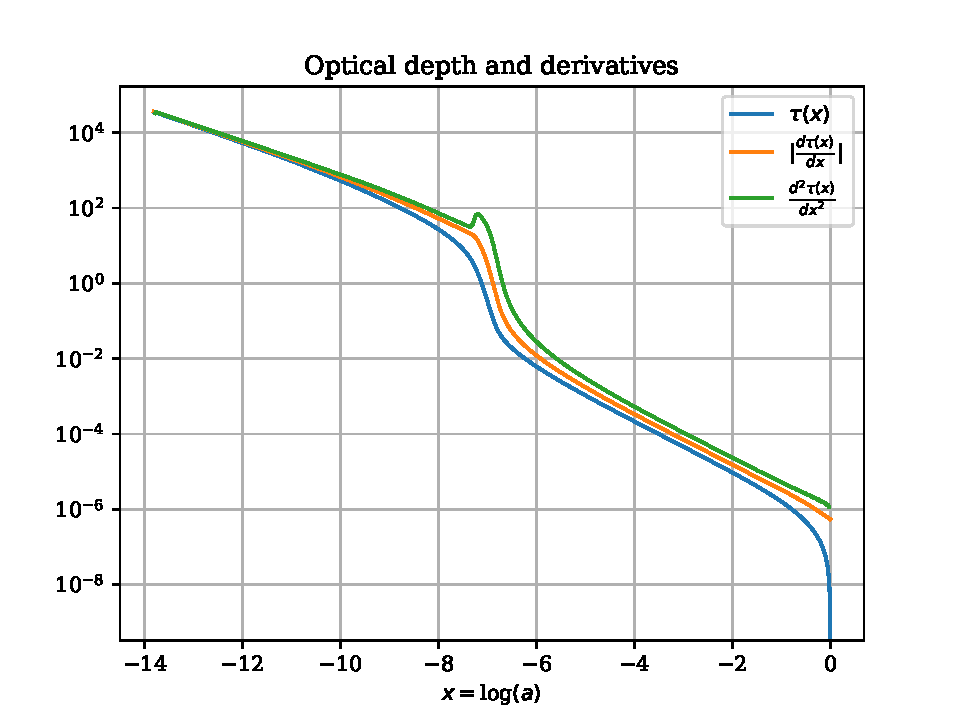
\includegraphics[scale=0.8]{figures/tau.pdf}
    \caption{Figure showing the optical depth of the universe $\tau$ and its derivatives as a function of $x=log(a)$.}S
    \label{fig:tau}
\end{figure}

\begin{figure}
    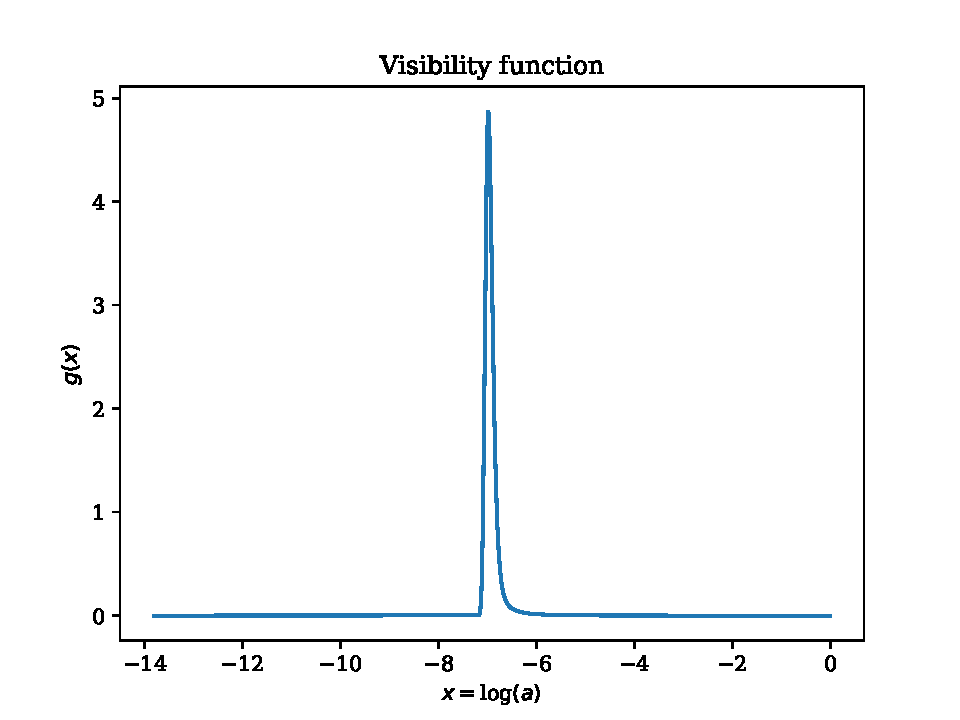
\includegraphics[scale=0.8]{figures/g.pdf}
    \caption{Figure showing the visibility function $\widetilde{g}(x)$ as a function of $x=log(a)$.}
    \label{fig:g}
\end{figure}

\begin{figure}
    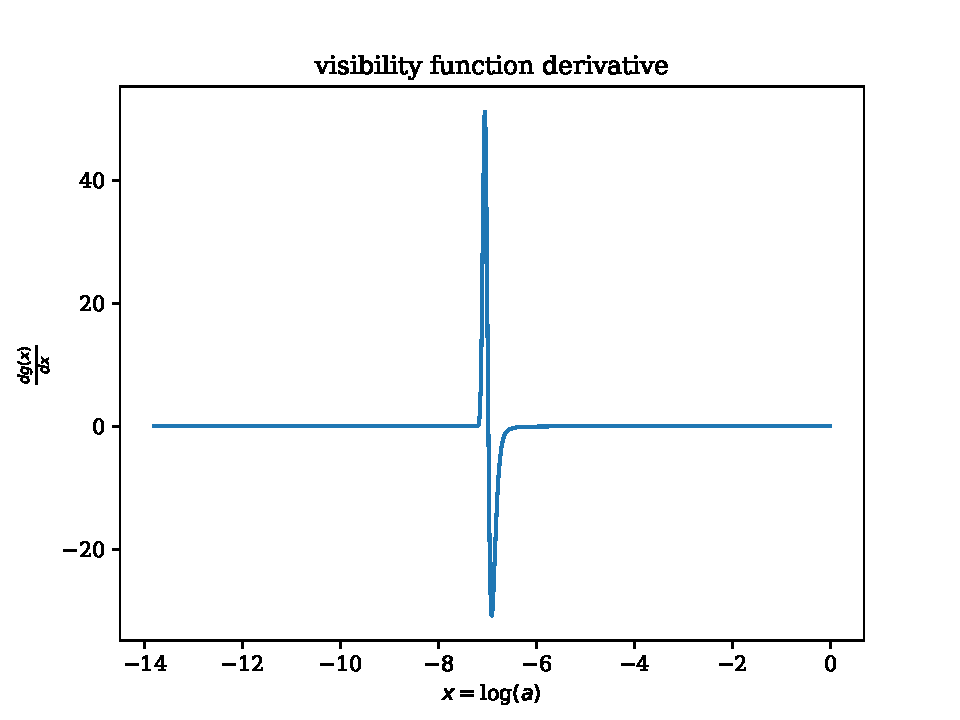
\includegraphics[scale=0.8]{figures/dgdx.pdf}
    \caption{Figure showing the derivative of the visibility function $\frac{d\widetilde{g}(x)}{dx}$ as a function of $x=log(a)$.}
    \label{fig:dgdx}
\end{figure}

\begin{figure}
    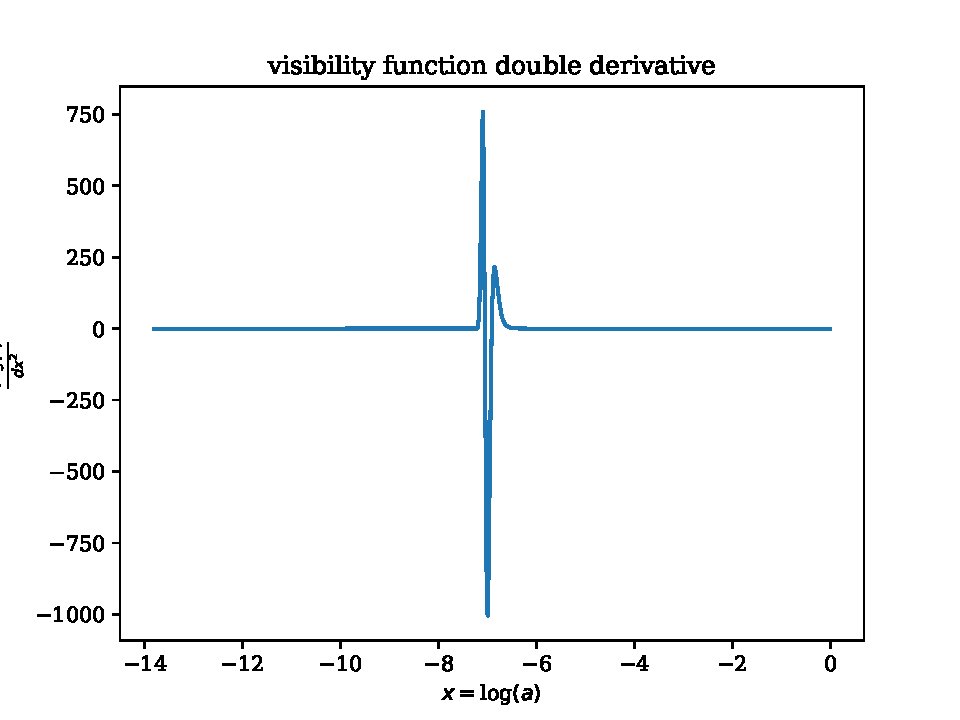
\includegraphics[scale=0.8]{figures/ddgdxx.pdf}
    \caption{Figure showing the double derivative of the visibility function $\frac{d^2\widetilde{g}(x)}{dx^2}$ as a function of $x=log(a)$.}
    \label{fig:ddgdxx}
\end{figure}
As a short benchmark the elapsed time for one random calculation of $X_e$ turned out be $0.00549402$ sec and for $\tau$ the elapsed time was $0.000820157$ sec. All timed with the C++ Chrono library.
\section{Discussion}\label{sec:discussion}
When studying the solution for the free electron fraction, as shown in figure \ref{fig:xe}, one can clearly see that in the early universe all electrons are free. The equilibrium solution from the Saha equation is valid until approximately $x=7.5$. At this time the equilibrium solution is no longer valid as photons decoupled due to the expansion of the universe. This allows protons and electron to combine and form neutral hydrogen. The results of our simulations also point to recombination and the last scattering happening shortly after this. Shortly after, electrons freeze out and stabilize at a constant fraction of around $X_e\approx10^{-4}$ making almost all baryonic matter in the universe neutral. By studying the number density of free electrons, as shown in figure \ref{fig:ne}, one can see that the number density experiences a sudden drop around the same time as recombination. Before this the number density falls of exponentially proportional to $a^{-3}$ After recombination, when the free electron fraction stays constant again, the number density of electrons falls off proportional to $a^{-3}$ again.



\bibliography{ref.bib}
\bibliographystyle{aasjournal}
%\begin{thebibliography}{}
%\end{thebibliography}
\end{document}

% End of file `sample62.tex'.
